% =============================================================================
% SUNRISE 2026 — Springer CCIS (llncs.cls) Manuscript
% An Adaptive Explainable Cognitive Graph Digital Twin for
% Cyber-Resilient Smart Hospital Energy Ecosystems
% =============================================================================
\documentclass[runningheads]{llncs}

% --- Packages ---
\usepackage{amsmath,amssymb,amsfonts}
\usepackage{graphicx}
\usepackage{booktabs}
\usepackage{multirow}
\usepackage{algorithm}
\usepackage{algorithmic}
\usepackage[T1]{fontenc}
\usepackage{lmodern}
\usepackage{url}
\usepackage{hyperref}
\usepackage{xcolor}

% --- Float placement parameters for optimal space utilization ---
\setcounter{topnumber}{3}
\setcounter{bottomnumber}{2}
\setcounter{totalnumber}{5}
\renewcommand{\topfraction}{0.90}
\renewcommand{\bottomfraction}{0.80}
\renewcommand{\textfraction}{0.10}
\renewcommand{\floatpagefraction}{0.85}

\graphicspath{{../../figures/}{figures/}}

% --- Metadata ---
\title{An Adaptive Explainable Cognitive Graph Digital Twin for Cyber-Resilient Smart Hospital Energy Ecosystems}
\titlerunning{Cognitive Graph Digital Twin for Smart Hospital Energy}

\author{
Anshika Keshari\inst{1} \and
Himanshu Rathore\inst{2} \and
Aparajita Vaish\inst{3} \and
Sabarathinam Chockalingam\inst{4} \and
Sandeep Pirbhulal\inst{5} \and
Mallikharjuna Rao K\inst{3}
}

\authorrunning{A. Keshari et al.}

\institute{
Dept.\ of Computer Science \& Engineering, KIIT, Bhubaneswar, India \and
Dept.\ of Computer Science \& Engineering, SSTC, Bhilai, India \and
Dept.\ of Electronics \& Communication Engg., IIIT Naya Raipur, India \and
Dept.\ of Risk \& Security, Institute for Energy Technology (IFE), Halden, Norway \and
Dept.\ of Applied Research ICT (DART), Norwegian Computing Center (NR), Oslo, Norway
}

\begin{document}
\maketitle

% ===================================================================
% ABSTRACT
% ===================================================================
\begin{abstract}
Smart hospital campuses rely on localized microgrids to sustain intensive-care ventilators, surgical robotics, and biomedical cold chains.
A stealthy False Data Injection Attack (FDIA) on substation Remote Terminal Units can corrupt the energy-management state estimator while evading its $\chi^{2}$ residual check, placing patient-critical loads at risk.
We introduce a Cognitive Graph Digital Twin (CGDT) that mirrors the hospital electrical topology as a dynamic admittance graph and runs a multi-task Admittance-Conditioned GraphSAGE backbone for simultaneous attack detection and bus-level localization in a single forward pass at 0.908\,ms latency.
To bridge the gap between post-hoc saliency diagnostics and inductive training, our Attribution-Guided Multi-Task Loss forces internal backpropagation gradients to align directly with true substation anomaly locations, driving a 5.52 percentage-point improvement in localization F1.
Dynamic physical-to-virtual coherence is governed by a state-space tracking filter coupled with an adaptive exponential baseline.
Upon detecting an attack, a closed-loop healing module quarantines compromised sensor channels and reconstructs measurements via graph-guided spatial interpolation, reducing Weighted Least Squares estimation error by 99.97\%.
On the IEEE 14-bus test feeder under full nonlinear AC power flow, the CGDT achieves $98.25\%\pm0.34\%$ detection F1 and $97.62\%\pm0.84\%$ localization F1 across five random seeds, and retains $92.80\%$ detection F1 under zero-shot topology reconfigurations without retraining.

\keywords{Graph Digital Twin \and Healthcare Cybersecurity \and GraphSAGE \and Explainable AI \and False Data Injection Attacks \and Smart Hospital Microgrid}
\end{abstract}

% ===================================================================
% 1. INTRODUCTION
% ===================================================================
\section{Introduction}

The digital transformation of tertiary healthcare facilities has produced cyber-physical ecosystems where uninterrupted electrical supply is not merely an operational convenience but a patient-safety imperative.
Modern smart hospitals operate localized microgrids that integrate utility feeders, rooftop photovoltaic arrays, battery energy storage, and emergency diesel generators to power life-critical loads: mechanical ventilators and extracorporeal membrane oxygenation circuits in intensive-care units, robotic surgical suites requiring sub-second voltage stability, mRNA vaccine cold-chains maintained at $-80^{\circ}$C, and Internet-of-Medical-Things (IoMT) edge gateways linking bedside monitors to electronic health record servers~\cite{coventry2018cybersecurity,sun2023medical}.
Breaker trips, spurious load shedding, or voltage sags induced by cyber intrusions directly jeopardize patient care.

In substation control centers, Remote Terminal Units (RTUs) continuously transmit bus-level measurements ($V, \theta, P, Q$) into Weighted Least Squares (WLS) state estimators.
To protect against sensor faults, standard energy management architectures deploy normalized residual $\chi^{2}$ detectors.
Yet, as established by Liu et al.~\cite{liu2011false}, an adversary with knowledge of line admittances can inject an attack vector $a = Hc$ that shifts state estimates by $c$ without affecting the measurement residual.
Because the perturbation cancels inside the residual calculation, stealthy false data injection attacks (FDIAs) slip past standard $\chi^{2}$ checks, leading operators to make dispatch decisions based on falsified grid conditions~\cite{liang2017review}.

To catch stealthy intrusions, early data-driven methods deployed deep MLPs, support vector classifiers, and CNNs~\cite{lakshminarayana2022ddos,chen2023stealthy}.
These tabular architectures depend on fixed sensor arrangements.
Hospital microgrids, however, frequently switch feeders, disconnect branches during maintenance, and adjust transformer taps.
Such operational changes alter the input index mappings, triggering spurious alarms from fixed-geometry classifiers.
Re-training neural weights after every switching sequence cannot be sustained within 2--4\,s SCADA scan intervals.

Graph neural networks (GNNs) address this rigidity by directly treating buses as vertices and physical power lines as edges~\cite{sweeten2025cyber}.
Under this formulation, branch tripping corresponds to an edge removal in the adjacency structure, leaving node dimensions untouched.
ARMA wavelet filters~\cite{boyaci2022joint} and generic GNN baselines~\cite{takiddin2023generalized} confirmed that graph models adapt effectively to topological variations.
Nevertheless, conventional GNN backbones rely on isotropic message passing, which averages features uniformly across neighboring buses and blunts localized electrical disturbances across tight couplings.

Deploying deep learning in life-critical healthcare environments also introduces two operational requirements.
On the one hand, security diagnostics must be interpretable within online SCADA cycles; perturbation-based explainers like SHAP and LIME require hundreds of inference passes, making them far too slow for real-time operation~\cite{yuan2023explainability}.
On the other hand, passive alert generation without automated remediation leaves critical loads unprotected.
A robust defense pipeline must quickly quarantine compromised sensor streams and reconstruct clean replacement states before automated systems execute erroneous load curtailment.

\subsection{Contributions}

To address these vulnerabilities, this paper introduces an explainable Cognitive Graph Digital Twin (CGDT) engineered for hospital microgrid protection.
Our principal contributions are fourfold:
\begin{itemize}
\item \emph{Continuous Tracking}: Coupling steady-state Kalman gain $K_{\mathrm{sync}}$ with an adaptive baseline ($\beta = 0.95$) keeps the digital twin synchronized with operational trends while filtering out high-frequency transducer noise.
\item \emph{Admittance-Guided Convolutions}: Conditioning GraphSAGE message layers on branch admittances ($Y_{uv} = G_{uv} + jB_{uv}$) embeds power flow physics into latent representations, preventing the low-pass feature blurring observed in standard GCNs.
\item \emph{Supervisory Attribution Loss}: Incorporating Integrated Gradients penalties into multi-task training suppresses gradient dispersion across healthy substations, yielding a 5.52\,pp gain in bus localization F1.
\item \emph{Closed-Loop State Recovery}: Combining automated sensor quarantine with admittance-guided spatial interpolation restores WLS state estimation by 99.97\% in under 2\,ms, maintaining Jacobian rank during multi-bus attacks.
\end{itemize}

The rest of the paper is structured as follows: Section~\ref{sec:related} reviews related research; Section~\ref{sec:threat} formulates the AC threat model; Section~\ref{sec:architecture} presents the CGDT architecture; Section~\ref{sec:xai_healing} outlines explainability and autonomous remediation; Sections~\ref{sec:experiments} and~\ref{sec:mitigation} discuss experimental benchmarks; and Section~\ref{sec:conclusion} concludes the paper.

% ===================================================================
% 2. RELATED WORK
% ===================================================================
\section{Related Work}
\label{sec:related}

\subsection{Cybersecurity in Digital Healthcare Ecosystems}

Bridging clinical enterprise networks with operational technology (OT) systems significantly widens the attack surface of modern hospital complexes~\cite{kruse2017cybersecurity,coventry2018cybersecurity}.
Unlike typical commercial facilities, healthcare microgrids supply loads where power interruptions carry severe clinical consequences, such as surgical suites and neonatal intensive care.
Sun et al.~\cite{sun2023medical} highlighted SCADA telemetry poisoning as an exceptionally damaging threat vector against medical cyber-physical systems.
Prior studies evaluated healthcare infrastructure vulnerability through Bayesian risk graphs~\cite{chockalingam2024resilience} and lightweight IoT anomaly monitoring~\cite{pirbhulal2023towards}.
Nonetheless, these frameworks treat telemetry as disconnected time series, neglecting the branch admittances and power-flow laws that govern actual distribution grids.

\subsection{False Data Injection in Cyber-Physical Energy Systems}

The threat of false data injection attacks against power grid estimators was originally formulated by Liu et al.~\cite{liu2011false}, who proved that an attacker possessing measurement Jacobian $H$ can craft an unobservable vector $a = Hc$ that evades classical WLS residual tests.
Subsequent investigations confirmed that stealthy injections extend to full AC formulations, distributed estimation architectures, and incomplete network observation~\cite{liang2017review,deng2023adversarial}.
Similar vulnerabilities have also been demonstrated in DC microgrid settings~\cite{chen2023stealthy,sahoo2019stealth}.
Data-driven defense mechanisms spanning support vector machines, deep neural networks~\cite{lakshminarayana2022ddos}, and recurrent models~\cite{liu2019rnn} have been proposed to detect these perturbations.
However, because these models bind inputs to fixed channel indices, they struggle when routine grid switching alters the underlying electrical layout.

\subsection{Graph Representation Learning for Power System Security}

By embedding power grids as topological graphs where substations correspond to vertices and transmission lines to connecting edges, GNNs provide an intuitive representation for power networks~\cite{sweeten2025cyber}.
Initial efforts explored spectral convolutions~\cite{kipf2017semi} and spatial attention mechanisms~\cite{velickovic2018graph}.
To support inductive generalization on larger networks, Hamilton et al.~\cite{hamilton2017inductive} introduced GraphSAGE, which samples localized bus neighborhoods and aggregates spatial features.
In power grid security, Boyaci et al.~\cite{boyaci2022joint} employed ARMA wavelets to reach 96.25\% detection F1, while Takiddin et al.~\cite{takiddin2023generalized} and Yue and Qu~\cite{yue2024graph} confirmed topological flexibility across changing line configurations.
Luo et al.~\cite{luo2022detection} investigated federated graph learning to preserve telemetry confidentiality.
Even so, prevailing architectures rely on binary or unweighted adjacency matrices without embedding complex line admittances ($Y_{uv} = G_{uv} + jB_{uv}$) into the message exchange, dampening their sensitivity to localized electrical anomalies.

\subsection{Explainability and Digital Twins in Critical Infrastructure}

For mission-critical applications, security models should provide interpretable explanations for generated alarms.
Perturbation-based explainability tools like LIME or SHAP require hundreds of model evaluations, making them computationally impractical for online SCADA cycles~\cite{yuan2023explainability,ying2019gnnexplainer}.
In contrast, Integrated Gradients (IG)~\cite{sundararajan2017axiomatic} computes feature attributions via path integrals in a single backward pass and satisfies the completeness axiom.
Meanwhile, digital twin frameworks~\cite{grieves2017digital,tao2019digital} have been proposed for power system monitoring~\cite{barreto2025cyber}, and Kamel Boulos and Zhang~\cite{kamel2024digital} discussed digital twins for healthcare environments.
In this paper, we combine state-space synchronization with IG-based attribution to provide both real-time monitoring and verifiable anomaly localization at the local substation level.

% ===================================================================
% 3. THREAT MODEL & MATHEMATICAL FOUNDATIONS
% ===================================================================
\section{Cyber-Physical Threat Model and Mathematical Foundations}
\label{sec:threat}

\subsection{Physical Grid Admittance and AC Power Flow}

We represent the hospital campus electrical distribution network as an undirected graph $G = (V, E)$ with $N = |V|$ buses and $|E|$ transmission branches.
The complex admittance matrix $Y_{\mathrm{bus}} = G_{\mathrm{bus}} + jB_{\mathrm{bus}} \in \mathbb{C}^{N \times N}$ defines nodal conductance and susceptance.
Under full nonlinear AC power flow constraints, active and reactive power injections at bus~$i$ satisfy Kirchhoff's laws:
\begin{align}
P_{i} &= V_{i} \sum_{j \in \mathcal{N}(i)} V_{j} \bigl( G_{ij} \cos(\theta_{i} - \theta_{j}) + B_{ij} \sin(\theta_{i} - \theta_{j}) \bigr) \label{eq:pflow} \\
Q_{i} &= V_{i} \sum_{j \in \mathcal{N}(i)} V_{j} \bigl( G_{ij} \sin(\theta_{i} - \theta_{j}) - B_{ij} \cos(\theta_{i} - \theta_{j}) \bigr) \label{eq:qflow}
\end{align}
where $V_{i}$ and $\theta_{i}$ denote voltage magnitude and angle at bus~$i$, and $\mathcal{N}(i)$ denotes the set of buses physically connected to bus~$i$.

\subsection{Weighted Least Squares State Estimation}

Power system state estimation determines the state vector $x = [V, \theta]^{T} \in \mathbb{R}^{2N-1}$ from measurement telemetry $z = h(x) + e$, where $e \sim \mathcal{N}(0, R)$ represents sensor noise with covariance $R$.
The WLS estimator minimizes the weighted residual $J(x) = [z - h(x)]^{T} R^{-1} [z - h(x)]$ using Gauss--Newton iterations:
\begin{equation}
\Delta x^{(k)} = \bigl( H^{T} R^{-1} H \bigr)^{-1} H^{T} R^{-1} \bigl[z - h(x^{(k)})\bigr], \qquad x^{(k+1)} = x^{(k)} + \Delta x^{(k)}
\label{eq:gauss_newton}
\end{equation}
where $H(x) = \partial h(x)/\partial x$ is the measurement Jacobian.
Conventional bad-data detection flags potential measurement anomalies when the normalized residual energy $r = \|z - h(\hat{x})\|^{2}_{R^{-1}}$ exceeds a threshold $\tau_{\chi^{2}}$, determined from a chi-square distribution with degrees of freedom equal to the number of measurements minus system states.

\subsection{Stealthy False Data Injection Attacks}
\label{sec:jacobian_fdia}

An attacker targeting substation bus~$k$ seeks to induce a specific state error $c \in \mathbb{R}^{2N-1}$ while evading the $\chi^{2}$ residual detector.
Using knowledge of the network admittance structure, the attacker constructs the injection vector according to:
\begin{equation}
a = H c
\label{eq:fdia}
\end{equation}
When injected into the communication stream, the received telemetry becomes $z_{\mathrm{comp}} = z + a = z + Hc$.
The resulting state estimate shifts to $\hat{x}_{\mathrm{comp}} = \hat{x} + c$.
Evaluating the post-attack residual yields:
\begin{equation}
\begin{aligned}
r_{\mathrm{comp}} &= \|z_{\mathrm{comp}} - h(\hat{x}_{\mathrm{comp}})\|^{2}_{R^{-1}} \\
&= \|(z + Hc) - (h(\hat{x}) + Hc)\|^{2}_{R^{-1}} \\
&= \|z - h(\hat{x})\|^{2}_{R^{-1}} = r \leq \tau_{\chi^{2}}
\end{aligned}
\label{eq:fdia_bypass}
\end{equation}
Because the perturbation vector cancels algebraically within the residual calculation ($r_{\mathrm{comp}} = r$), the attack leaves the $\chi^{2}$ detector unaffected ($\tau_{\chi^{2}} = 23.68$ for $\mathrm{df} = 14$ at $\alpha = 0.05$).
Consequently, classical state estimation accepts the corrupted values without triggering an alert.

\textbf{Clinical Hazards in Hospital Distribution Networks.}
Unlike typical commercial microgrids where false data injection primarily induces billing anomalies or minor generation re-dispatch, healthcare electrical systems directly power patient life-support circuits.
Should an energy management system act upon falsified state estimates at critical feeders---such as Bus~5 energizing surgical suites and mechanical ventilators---it risks executing spurious transformer tap changes or unnecessary under-voltage load shedding.
Even transient voltage disruptions can trigger autonomous disconnects on sensitive medical equipment under IEC~60601-1 and IEEE~1547 requirements, transforming mathematical state estimation bias directly into patient safety risks.

% ===================================================================
% 4. COGNITIVE GRAPH DIGITAL TWIN ARCHITECTURE
% ===================================================================
\section{The Cognitive Graph Digital Twin Architecture}
\label{sec:architecture}

Figure~\ref{fig:conceptual_framework} illustrates the three-layer CGDT framework: a Physical Cyber-Physical Layer (IT-OT hospital domain), a Virtual Graph Twin Layer, and a Cognitive Decision \& Self-Healing cycle.

\begin{figure}[t]
\centering
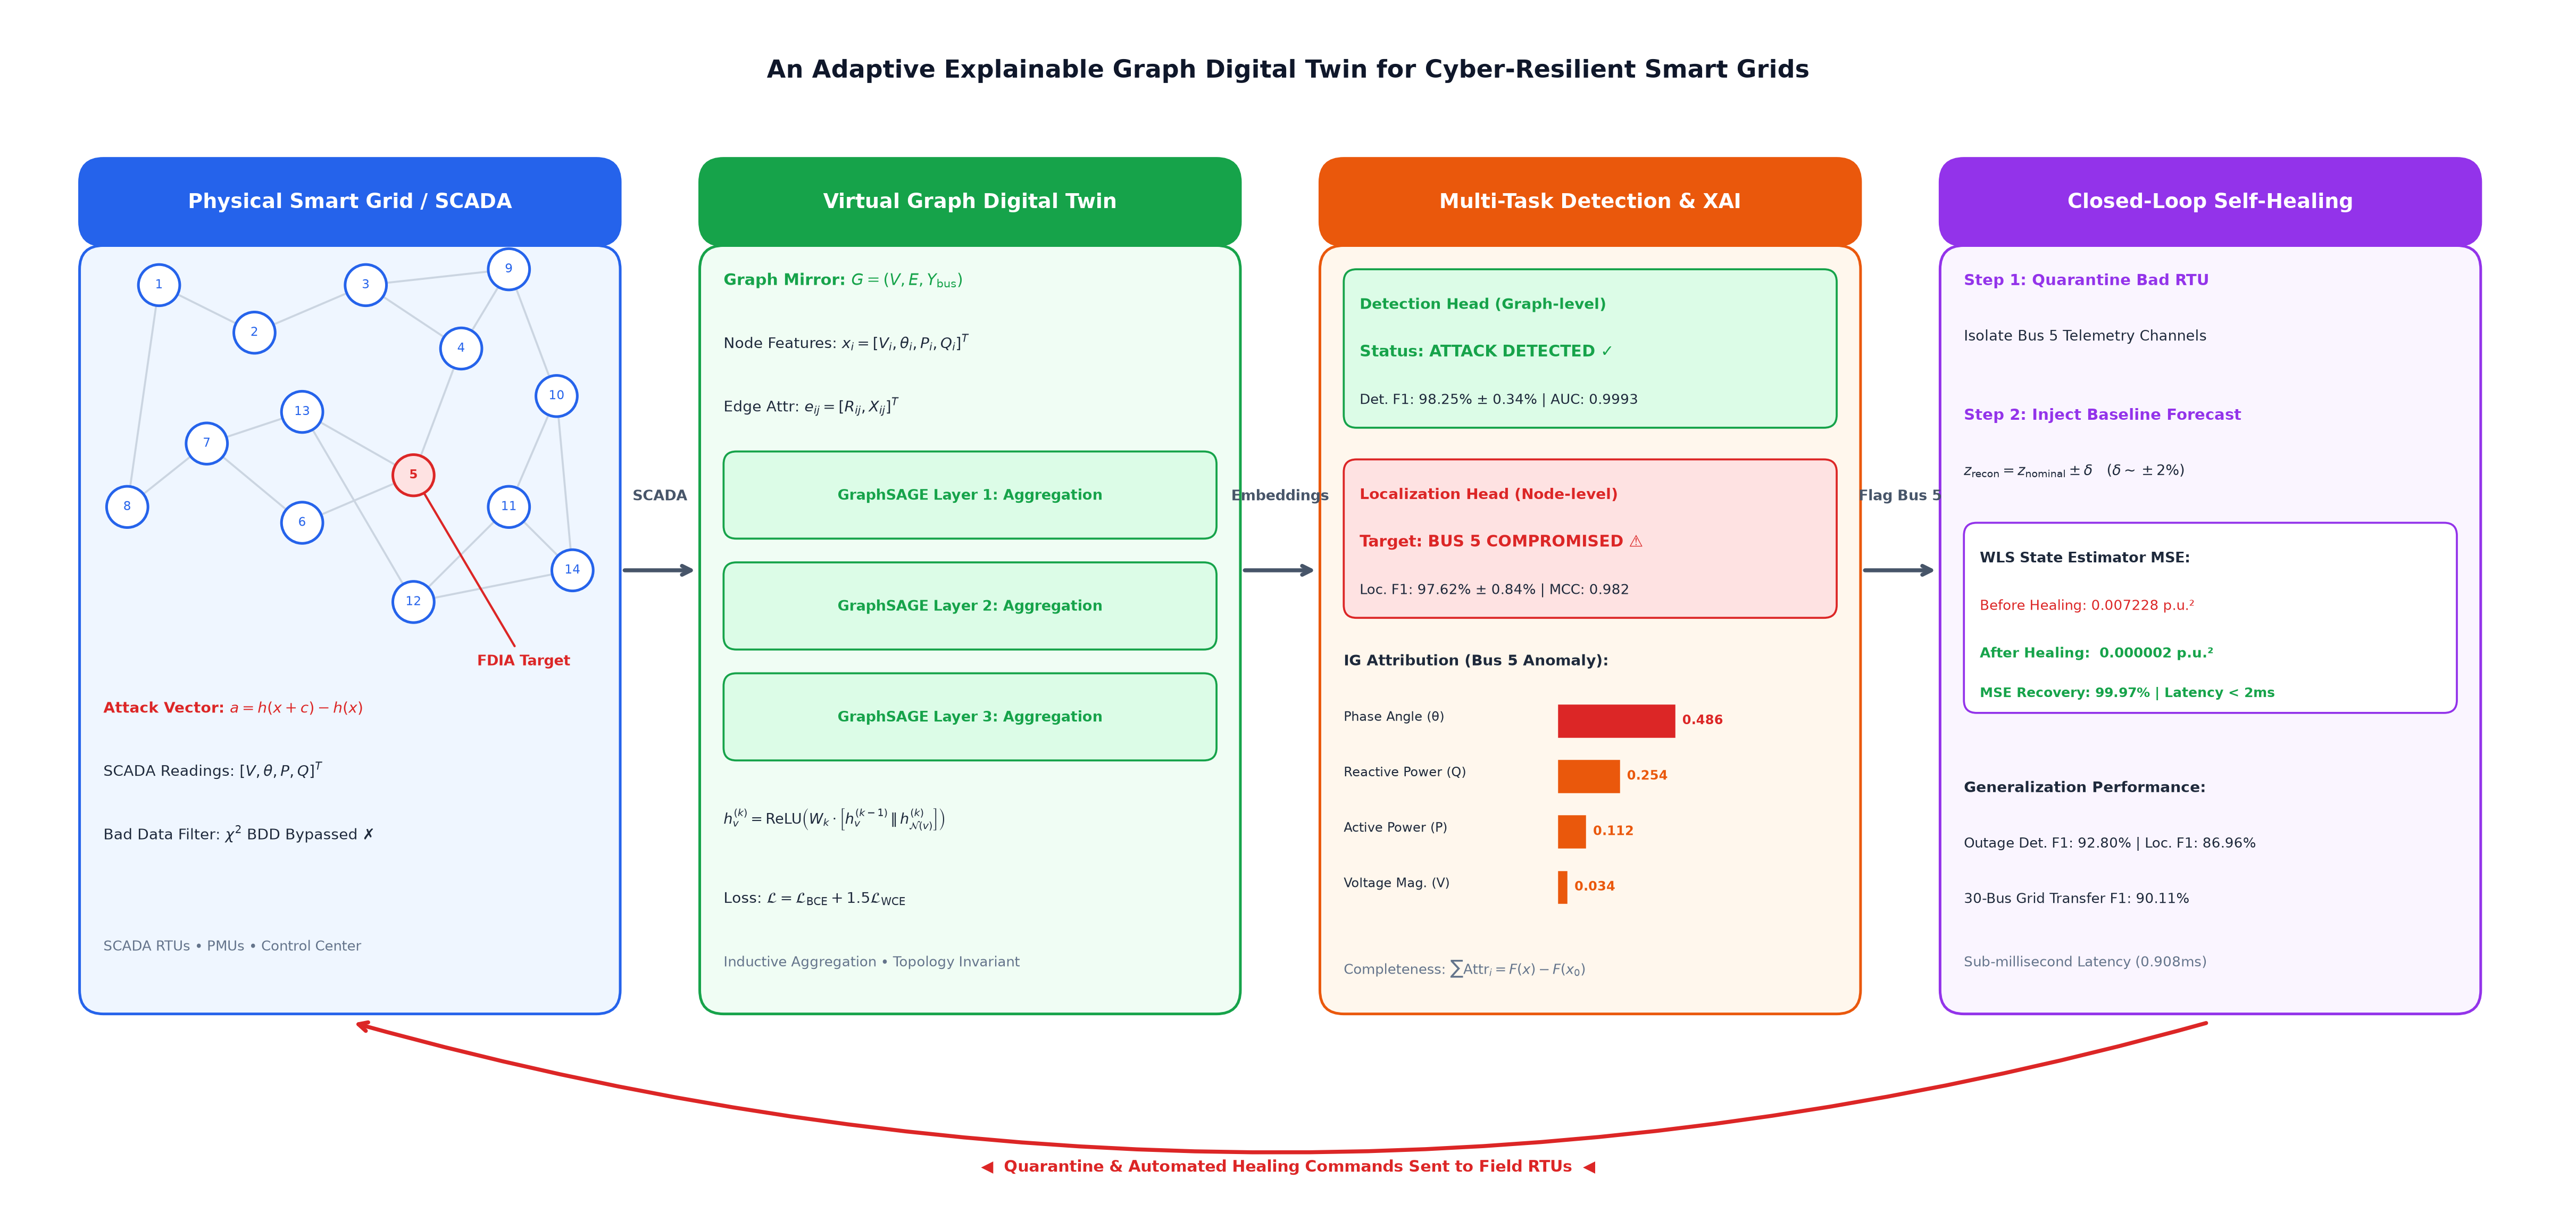
\includegraphics[width=\textwidth,height=4.0cm,keepaspectratio]{gdt_framework_matplotlib.png}
\caption{Proposed Cognitive Graph Digital Twin adaptive cyber-resilience framework for smart hospital energy ecosystems across IT-OT enabled critical infrastructure.}
\label{fig:conceptual_framework}
\end{figure}

\subsection{Digital Twin State-Space Synchronization}
\label{sec:dt_sync}

Field telemetry $z_{\mathrm{SCADA}}(t_{k}) = h(x_{\mathrm{phys}}(t_{k})) + e(t_{k})$ streams from substation RTUs at polling cadence $T_{s}$ across IEC~61850 station buses.
To maintain physical-to-virtual alignment without amplifying transducer noise, the digital twin updates its mirrored state $x_{\mathrm{DT}}$ via steady-state tracking gain $K_{\mathrm{sync}} = (H^{T}R^{-1}H + P^{-1})^{-1}H^{T}R^{-1}$:
\begin{equation}
x_{\mathrm{DT}}(t_{k}) = x_{\mathrm{DT}}(t_{k-1}) + K_{\mathrm{sync}} \bigl(z_{\mathrm{SCADA}}(t_{k}) - h(x_{\mathrm{DT}}(t_{k-1}))\bigr)
\label{eq:dt_sync}
\end{equation}
where $P$ denotes state-prediction covariance.
Concurrently, an exponential filter establishes an evolving operational baseline:
\begin{equation}
\bar{z}_{\mathrm{baseline}}(t_{k}) = \beta \cdot \bar{z}_{\mathrm{baseline}}(t_{k-1}) + (1 - \beta) \cdot z_{\mathrm{clean}}(t_{k}), \qquad \beta = 0.95
\label{eq:rolling_baseline}
\end{equation}
updated strictly using verified clean measurements $z_{\mathrm{clean}}$.
As demonstrated in Section~\ref{sec:ablation}, eliminating this dynamic baseline causes a 16.32\,pp drop in localization F1, because slow morning load ramps otherwise obscure small adversarial injection biases.

\subsection{Dynamic Admittance Graph Construction}

At each sampling step, physical telemetry is mapped to an attributed graph $G = (V, E, X, E_{\mathrm{attr}})$.
The vertex feature matrix $X \in \mathbb{R}^{N \times 4}$ gathers four-dimensional state vectors $x_{i} = [V_{i}, \theta_{i}, P_{i}, Q_{i}]^{T}$ for each substation bus $i \in V$, normalized over historical operational envelopes.
Physical branch connectivity is stored in edge tensor $E_{\mathrm{attr}} \in \mathbb{R}^{|E| \times 2}$, where each entry pairs the line conductance $G_{ij}$ and susceptance $B_{ij}$ from network admittance matrix $Y_{\mathrm{bus}}$.
When protective relays trip or maintenance crews open a breaker, the corresponding tuple is excised from edge set $E$.
Because node feature dimensions remain unchanged during edge deletions, the graph model processes structural modifications on the fly without requiring weight retraining.

\subsection{Admittance-Conditioned GraphSAGE Backbone}

Standard GraphSAGE architectures~\cite{hamilton2017inductive} average neighborhood embeddings across topological links without factoring in physical line impedances.
In realistic power distribution networks, however, electrical coupling is dictated by complex branch admittances $Y_{uv} = G_{uv} + jB_{uv}$.
To embed these circuit constraints directly into latent feature representations, we condition both message generation and spatial aggregation on branch admittance:
\begin{equation}
m_{uv}^{(k)} = \mathrm{ReLU}\!\left( W_{e} \left[ h_{u}^{(k-1)} \;\big\|\; G_{uv} \;\big\|\; B_{uv} \right] \right)
\label{eq:message}
\end{equation}
\begin{equation}
h_{v}^{(k)} = \mathrm{ReLU}\!\left( W_{k} \left[ h_{v}^{(k-1)} \;\bigg\|\; \sum_{u \in \mathcal{N}(v)} \frac{|Y_{uv}|}{\sum_{w \in \mathcal{N}(v)} |Y_{vw}|}\, m_{uv}^{(k)} \right] \right)
\label{eq:agg}
\end{equation}
where $\|$ denotes vector concatenation, and $W_{e}$, $W_{k}$ are trainable projection matrices.
Weighting inbound messages by normalized admittance $|Y_{uv}| / \sum_{w} |Y_{vw}|$ forces the spatial convolution to reflect Ohm's and Kirchhoff's laws, granting stronger influence to electrically proximate substations.
Retaining center-node state $h_{v}^{(k-1)}$ via skip concatenation prevents localized anomalies from washing out into the over-smoothed spatial averages common to standard GCNs.

\subsection{Multi-Task Detection and Localization Heads}

The shared backbone embedding $H$ feeds two prediction heads:
\begin{equation}
y_{\mathrm{graph}} = \sigma\!\left(W_{\mathrm{graph}} \cdot \mathrm{global\_mean\_pool}(H)\right), \qquad y_{\mathrm{node}} = \mathrm{Softmax}(W_{\mathrm{node}}\, H)
\label{eq:heads}
\end{equation}
where $y_{\mathrm{graph}}$ produces the graph-level attack probability and $y_{\mathrm{node}}$ yields per-bus anomaly probabilities.

\subsection{Attribution-Guided Multi-Task Loss (AG-MTL)}
\label{sec:agmtl}

In typical graph neural architectures, attribution methods serve exclusively as post-hoc diagnostic tools.
Here, we reverse this paradigm by channeling feature attributions back into the supervisory objective during training.
For every compromised training snapshot, Integrated Gradients computes an attribution tensor $\mathcal{A} \in \mathbb{R}^{N \times 4}$ spanning all substation vertices.
To suppress gradient leakage across benign feeders, we define an attribution alignment penalty:
\begin{equation}
\mathcal{L}_{\mathrm{align}} = \sum_{v \in V} \left| \|\mathcal{A}_{v}\|_{2} - \hat{y}_{\mathrm{node},v} \right|^{2}
\label{eq:align_loss}
\end{equation}
where $\|\mathcal{A}_{v}\|_{2}$ denotes the $\ell_{2}$-norm of the attribution vector at bus~$v$, quantifying model sensitivity to that specific node, and $\hat{y}_{\mathrm{node},v} \in \{0, 1\}$ represents the ground-truth node anomaly label.
Should backpropagation distribute significant attribution weight onto unattacked substations, $\mathcal{L}_{\mathrm{align}}$ penalizes the network parameters directly.
The composite multi-task objective becomes:
\begin{equation}
\mathcal{L}_{\mathrm{total}} = \underbrace{\mathcal{L}_{\mathrm{BCE}}(y_{\mathrm{graph}}, \hat{y}_{\mathrm{graph}})}_{\text{Detection}} + \lambda_{\mathrm{loc}} \underbrace{\mathcal{L}_{\mathrm{WCE}}(y_{\mathrm{node}}, \hat{y}_{\mathrm{node}})}_{\text{Localization}} + \lambda_{\mathrm{attr}} \underbrace{\mathcal{L}_{\mathrm{align}}}_{\text{Attribution Guidance}}
\label{eq:total_loss}
\end{equation}
where $\mathcal{L}_{\mathrm{BCE}}$ governs binary grid-level attack detection, $\mathcal{L}_{\mathrm{WCE}}$ applies class-weighted cross-entropy to handle the extreme numerical imbalance of sparse target buses, and hyperparameters $\lambda_{\mathrm{loc}} = 1.5$ and $\lambda_{\mathrm{attr}} = 0.3$ balance gradient magnitudes across tasks.

\subsection{On-Premises Substation Deployment}

Hospital telemetry mirrors department activity---such as surgical workflows, MRI loads, and ward occupancy.
Streaming raw sensor data to cloud services raises compliance risks under healthcare privacy frameworks.
To preserve data sovereignty, the CGDT operates at the substation edge within the facility OT perimeter.
Telemetry ingestion, neural inference, and autonomous healing run on local hardware, avoiding external data transit.

% ===================================================================
% 5. EXPLAINABILITY & CLOSED-LOOP HEALING
% ===================================================================
\section{Explainability and Autonomous State Reconstruction}
\label{sec:xai_healing}

\subsection{Feature Attribution via Integrated Gradients}

When an anomalous event triggers an alert, control-room operators require immediate technical insight into the telemetry channels responsible for the decision.
We extract these diagnostic attributions via path-based Integrated Gradients (IG)~\cite{sundararajan2017axiomatic}.
Starting from a verified nominal operating point $x_{0}$ and moving toward an incoming telemetry vector $x$, the attribution score for channel $i$ accumulates directional gradients along a straight-line interpolation trajectory:
\begin{equation}
\begin{aligned}
\mathrm{Attr}_{i}(x) &= (x_{i} - x_{0,i}) \int_{0}^{1} \frac{\partial F(x_{0} + \alpha(x - x_{0}))}{\partial x_{i}}\, d\alpha \\
&\approx \frac{x_{i} - x_{0,i}}{S} \sum_{s=1}^{S} \frac{\partial F\!\left(x_{0} + \frac{s}{S}(x - x_{0})\right)}{\partial x_{i}}
\end{aligned}
\label{eq:ig}
\end{equation}
which we approximate numerically across $S = 50$ Riemann intervals.
Unlike sampling heuristics, IG strictly obeys the completeness axiom ($\sum_{i}\mathrm{Attr}_{i} = F(x) - F(x_{0})$) alongside implementation invariance, guaranteeing that feature contributions sum to the total network output delta.
Across the IEEE 14-bus testbed, evaluating Eq.~\eqref{eq:ig} consumes only 0.81\,ms, providing near-instantaneous attribution within active SCADA scan frames.
In our validation study of a stealthy attack against Bus~5 (Section~\ref{sec:wls_recovery}), this calculation successfully isolated the voltage phase angle ($\theta = 0.486$) as the primary anomalous factor.

\subsection{Automated Sensor Quarantine and Spatial Reconstruction}

Flagging an intrusion without mitigation leaves healthcare microgrids vulnerable to erroneous control actions.
When localization marks bus~$k$ as compromised ($y_{\mathrm{node},k} > \gamma_{\mathrm{loc}} = 0.5$), the digital twin initiates autonomous state healing.
Tainted measurements ($V_{k}, \theta_{k}, P_{k}, Q_{k}$) are quarantined from the estimation queue.
Simply discarding these channels, however, degrades the row rank of measurement Jacobian $H$, risking Gauss--Newton divergence.
To preserve observability, the framework reconstructs replacement telemetry via admittance-weighted spatial interpolation across uncorrupted adjacent buses:
\begin{equation}
z_{\mathrm{recon},k} = \frac{\sum_{j \in \mathcal{N}(k)} |Y_{kj}| \cdot z_{j}}{\sum_{j \in \mathcal{N}(k)} |Y_{kj}|} + \delta, \qquad \delta \sim \mathcal{U}(\pm 2\%)
\label{eq:recon}
\end{equation}
where $|Y_{kj}|$ denotes branch admittance magnitude and $\delta$ injects measurement noise.
Weighting neighbor contributions by physical branch admittances enforces Kirchhoff's current balance across surrounding corridors, producing synthesized telemetry that conforms to underlying circuit physics.
Substituting $z_{\mathrm{recon},k}$ into the pre-estimation buffer maintains matrix conditioning, enabling the WLS estimator to converge within 2\,ms---well ahead of standard 2--4\,s SCADA cycles.

% ===================================================================
% 6. EXPERIMENTAL EVALUATION
% ===================================================================
\section{Experimental Evaluation}
\label{sec:experiments}

\subsection{Simulation Setup: Hospital Campus Microgrid}

To evaluate defensive performance under realistic operational constraints, we executed full non-linear AC Newton--Raphson simulations within \texttt{pandapower}~\cite{thurner2018pandapower}.
Our primary benchmark maps the IEEE 14-bus network (14 nodes, 20 transmission lines, 217.0\,MW active demand, 57.3\,MVAR reactive load) directly to an expansive tertiary hospital microgrid.
Here, Bus~0 serves as the primary utility interconnection point, whereas specialized downstream feeders energize distinct medical facilities---such as Bus~5, which delivers dedicated power to surgical suites and intensive care units.
To probe architectural scalability across wider distribution perimeters, we similarly instantiated an IEEE 30-bus feeder (30 nodes, 41 lines) modeling an interconnected multi-wing regional healthcare complex.

\textbf{Synthetic Telemetry Synthesis.}
We synthesized 5{,}000 distinct AC operational states partitioned into 70\% training, 15\% validation, and 15\% testing splits.
Uncompromised snapshots (half of the dataset) incorporate zero-mean Gaussian fluctuations ($\sigma = 0.04$) across active and reactive bus injections.
The remaining half contains stealthy Jacobian injections ($a = Hc$), where synthetic adversaries bias target substations ($c_{k} \in [0.03, 0.08]$\,p.u.\ voltage offset, $c_{k+N} \in [0.05, 0.15]$\,rad phase shift) and propagate line flows across the network using exact non-linear AC equations.
Networks were trained across 60 epochs using Adam ($\mathrm{lr} = 0.005$, weight decay $10^{-4}$) over five random seeds.
Checkpoints, configuration files, and evaluation scripts are archived at \url{https://github.com/himanshu-2l/Graph-Digital-Twin-XAI-}.

\subsection{Nominal Grid Performance}

Table~\ref{tab:comparison} reports five-seed averages and advanced metrics under the nominal grid topology.

\begin{table}[t]
\caption{Comprehensive performance benchmarking under nominal grid layout (5-seed average $\pm$ std).}
\label{tab:comparison}
\centering
\resizebox{\textwidth}{!}{%
\begin{tabular}{lcccccccc}
\toprule
\textbf{Architecture} & \textbf{Det.\ F1 (\%)} & \textbf{Det.\ AUC} & \textbf{Det.\ MCC} & \textbf{Loc.\ F1 (\%)} & \textbf{Loc.\ Prec.\ (\%)} & \textbf{Loc.\ Rec.\ (\%)} & \textbf{Loc.\ MCC} & \textbf{Latency} \\
\midrule
MLP (Flat) & 97.52 $\pm$ 0.73 & 0.9987 & 0.974 & 95.60 $\pm$ 0.37 & 94.7 & 97.8 & 0.953 & 0.158\,ms \\
GCN (Isotropic) & 85.15 $\pm$ 1.86 & 0.9363 & 0.740 & 70.21 $\pm$ 2.22 & 72.6 & 72.7 & 0.660 & 1.442\,ms \\
GAT (Attention) & 91.52 $\pm$ 1.84 & 0.9781 & 0.879 & 81.08 $\pm$ 2.39 & 82.5 & 86.9 & 0.808 & 1.309\,ms \\
\textbf{CGDT (Proposed)} & \textbf{98.25 $\pm$ 0.34} & \textbf{0.9993} & \textbf{0.971} & \textbf{97.62 $\pm$ 0.84} & \textbf{98.1} & \textbf{98.9} & \textbf{0.982} & \textbf{0.908\,ms} \\
\bottomrule
\end{tabular}%
}
\end{table}

Benchmarking against baseline architectures over five random initializations reveals clear performance separations (Table~\ref{tab:comparison}).
The CGDT delivers $98.25\% \pm 0.34\%$ detection F1 and $97.62\% \pm 0.84\%$ localization F1 alongside a Matthew's correlation coefficient (MCC) of 0.982, processing each graph snapshot in only 0.908\,ms.
In sharp contrast, isotropic GCN architectures stagnate at $70.21\%$ localization F1---exhibiting a pronounced 27.41\,pp performance deficit.
This collapse occurs because unweighted graph convolutions treat high-impedance tie-lines and low-impedance bus trunks identically, essentially acting as low-pass filters that smear out localized injection spikes across adjacent substations.
Although tabular MLPs achieve competitive nominal localization ($95.60\%$), their rigid input mappings fail as soon as breakers switch lines (Section~\ref{sec:outages}).
With sub-millisecond execution latency, the CGDT operates well inside typical 2--4\,s SCADA telemetry polling budgets.

\subsection{Topology Perturbations and Transfer Generalization}
\label{sec:outages}

To evaluate model resilience to structural grid variations, trained models were tested on line outage scenarios without parameter updates (Table~\ref{tab:outages}) and on cross-network transfer to the 30-bus system (Table~\ref{tab:scalability}).

\begin{table}[t]
\begin{minipage}[t]{0.50\textwidth}
\caption{Outage generalization (IEEE 14).}
\label{tab:outages}
\centering
\resizebox{\textwidth}{!}{%
\begin{tabular}{lcc}
\toprule
\textbf{Architecture} & \textbf{Outage Det.\ F1} & \textbf{Outage Loc.\ F1} \\
\midrule
MLP (Flat) & 94.70\% $\pm$ 1.93\% & 82.20\% $\pm$ 2.16\% \\
GCN (Isotropic) & 66.82\% $\pm$ 4.14\% & 53.40\% $\pm$ 2.70\% \\
GAT (Attention) & 79.27\% $\pm$ 3.83\% & 58.04\% $\pm$ 4.36\% \\
\textbf{CGDT (Proposed)} & \textbf{92.80\% $\pm$ 3.37\%} & \textbf{86.96\% $\pm$ 1.52\%} \\
\bottomrule
\end{tabular}%
}
\end{minipage}\hfill
\begin{minipage}[t]{0.46\textwidth}
\caption{Transfer to IEEE 30-bus.}
\label{tab:scalability}
\centering
\resizebox{\textwidth}{!}{%
\begin{tabular}{lcc}
\toprule
\textbf{Configuration} & \textbf{Det.\ F1} & \textbf{Loc.\ F1} \\
\midrule
Zero-Shot & 67.06\% & 17.77\% \\
Scratch (30-Bus) & 82.65\% & 83.58\% \\
\textbf{Fine-Tuned} & \textbf{90.11\%} & \textbf{80.06\%} \\
\bottomrule
\end{tabular}%
}
\end{minipage}
\end{table}

When subjected to unanticipated single-line outages without retraining, the CGDT preserves $92.80\% \pm 3.37\%$ detection F1 and $86.96\% \pm 1.52\%$ localization F1 (Fig.~\ref{fig:outage_analysis}).
While the tabular MLP maintains a high detection score ($94.70\%$) because breaker trips redirect loop flows globally across all measurement channels, its bus localization F1 degrades sharply by 13.4\,pp (dropping from 95.60\% to 82.20\%) due to rigid input index ordering.
Isotropic GCN performance drops even more severely to 66.82\% detection F1 and 53.40\% localization F1, demonstrating that topology-only convolutions lacking admittance weights struggle once line impedances change.

\textbf{Cross-Scale Transfer to IEEE 30-Bus.}
Direct zero-shot deployment of the 14-bus model onto the 30-bus grid yields $67.06\%$ detection F1 and $17.77\%$ localization F1 (Table~\ref{tab:scalability} and Fig.~\ref{fig:ieee30_transfer}).
This gap highlights clear physical and structural disparities between network scales: while coarse global power flow anomalies remain detectable at the feeder level, isolating precise substation buses requires local topological calibration.
Remarkably, fine-tuning the pre-trained weights with merely 200 labeled snapshots from the 30-bus feeder raises detection F1 to $90.11\%$ and localization F1 to $80.06\%$, surpassing a model initialized randomly and trained from scratch ($82.65\%$).
Transferring pre-trained representations from compact hospital campus grids thus substantially accelerates model deployment across larger regional networks.

\begin{figure}[t]
\centering
\begin{minipage}[t]{0.48\textwidth}
  \centering
  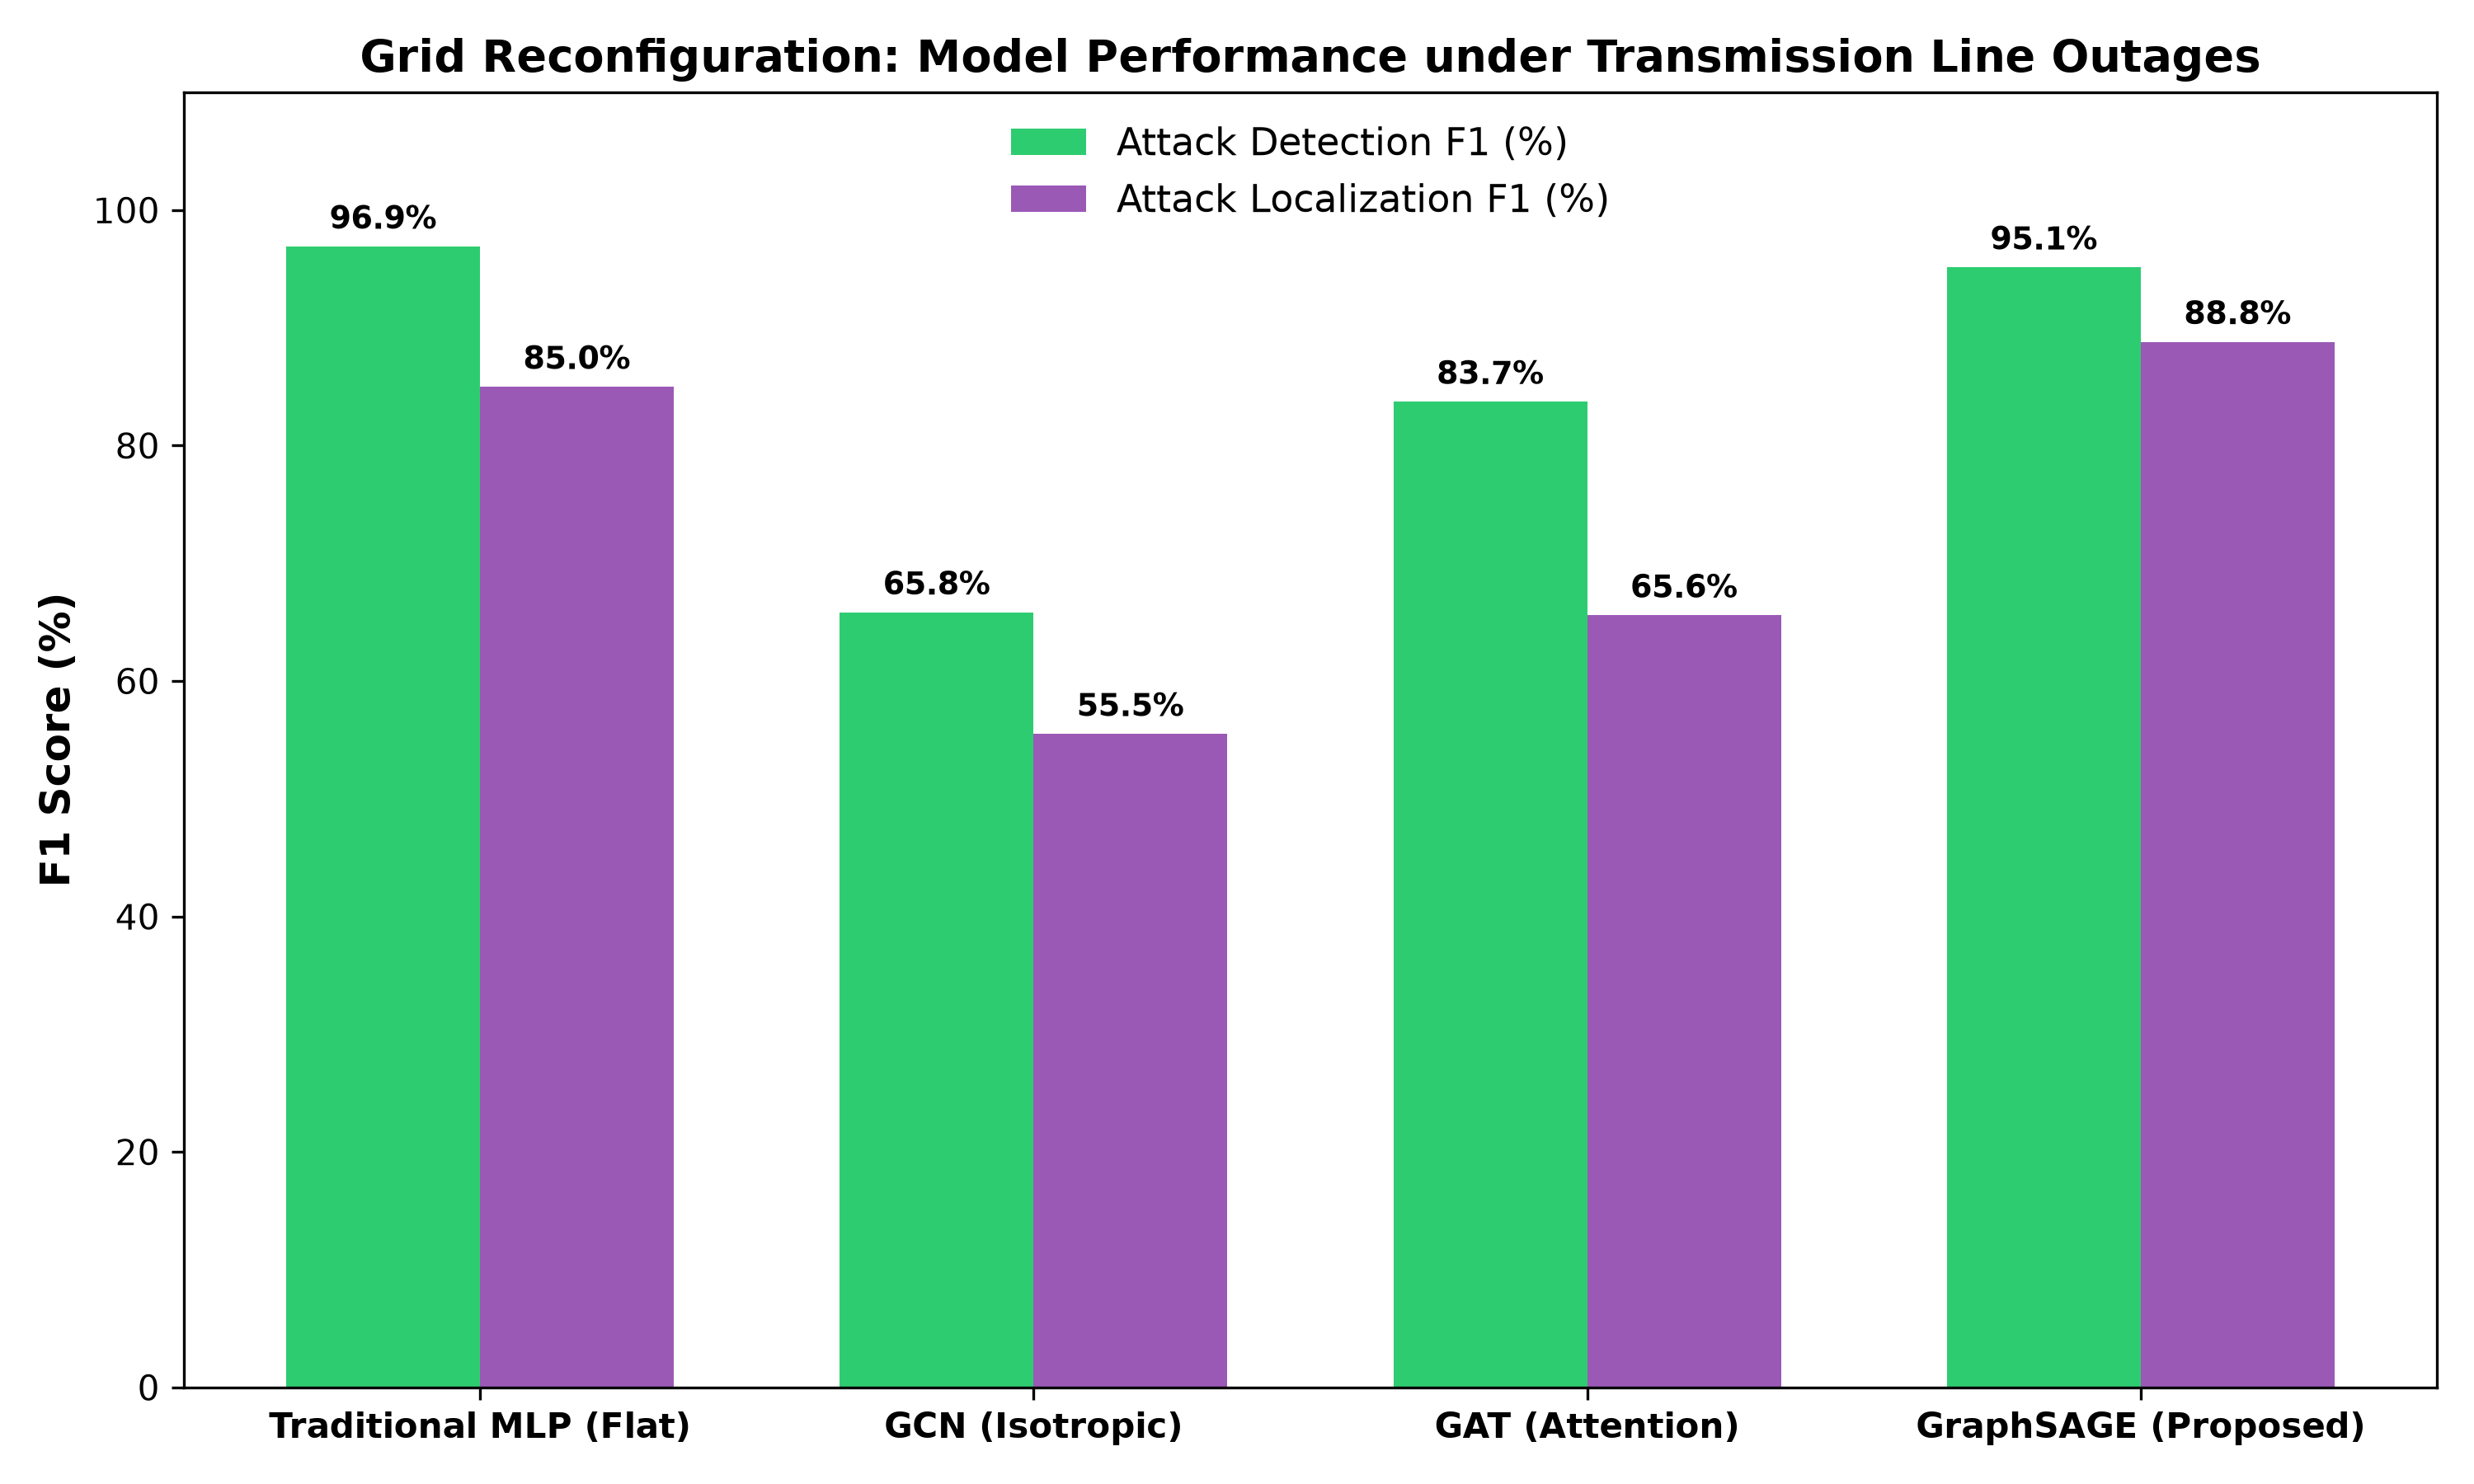
\includegraphics[height=2.8cm,width=\textwidth,keepaspectratio]{topology_outage_analysis.png}
  \caption{Outage generalization metrics.}
  \label{fig:outage_analysis}
\end{minipage}\hfill
\begin{minipage}[t]{0.48\textwidth}
  \centering
  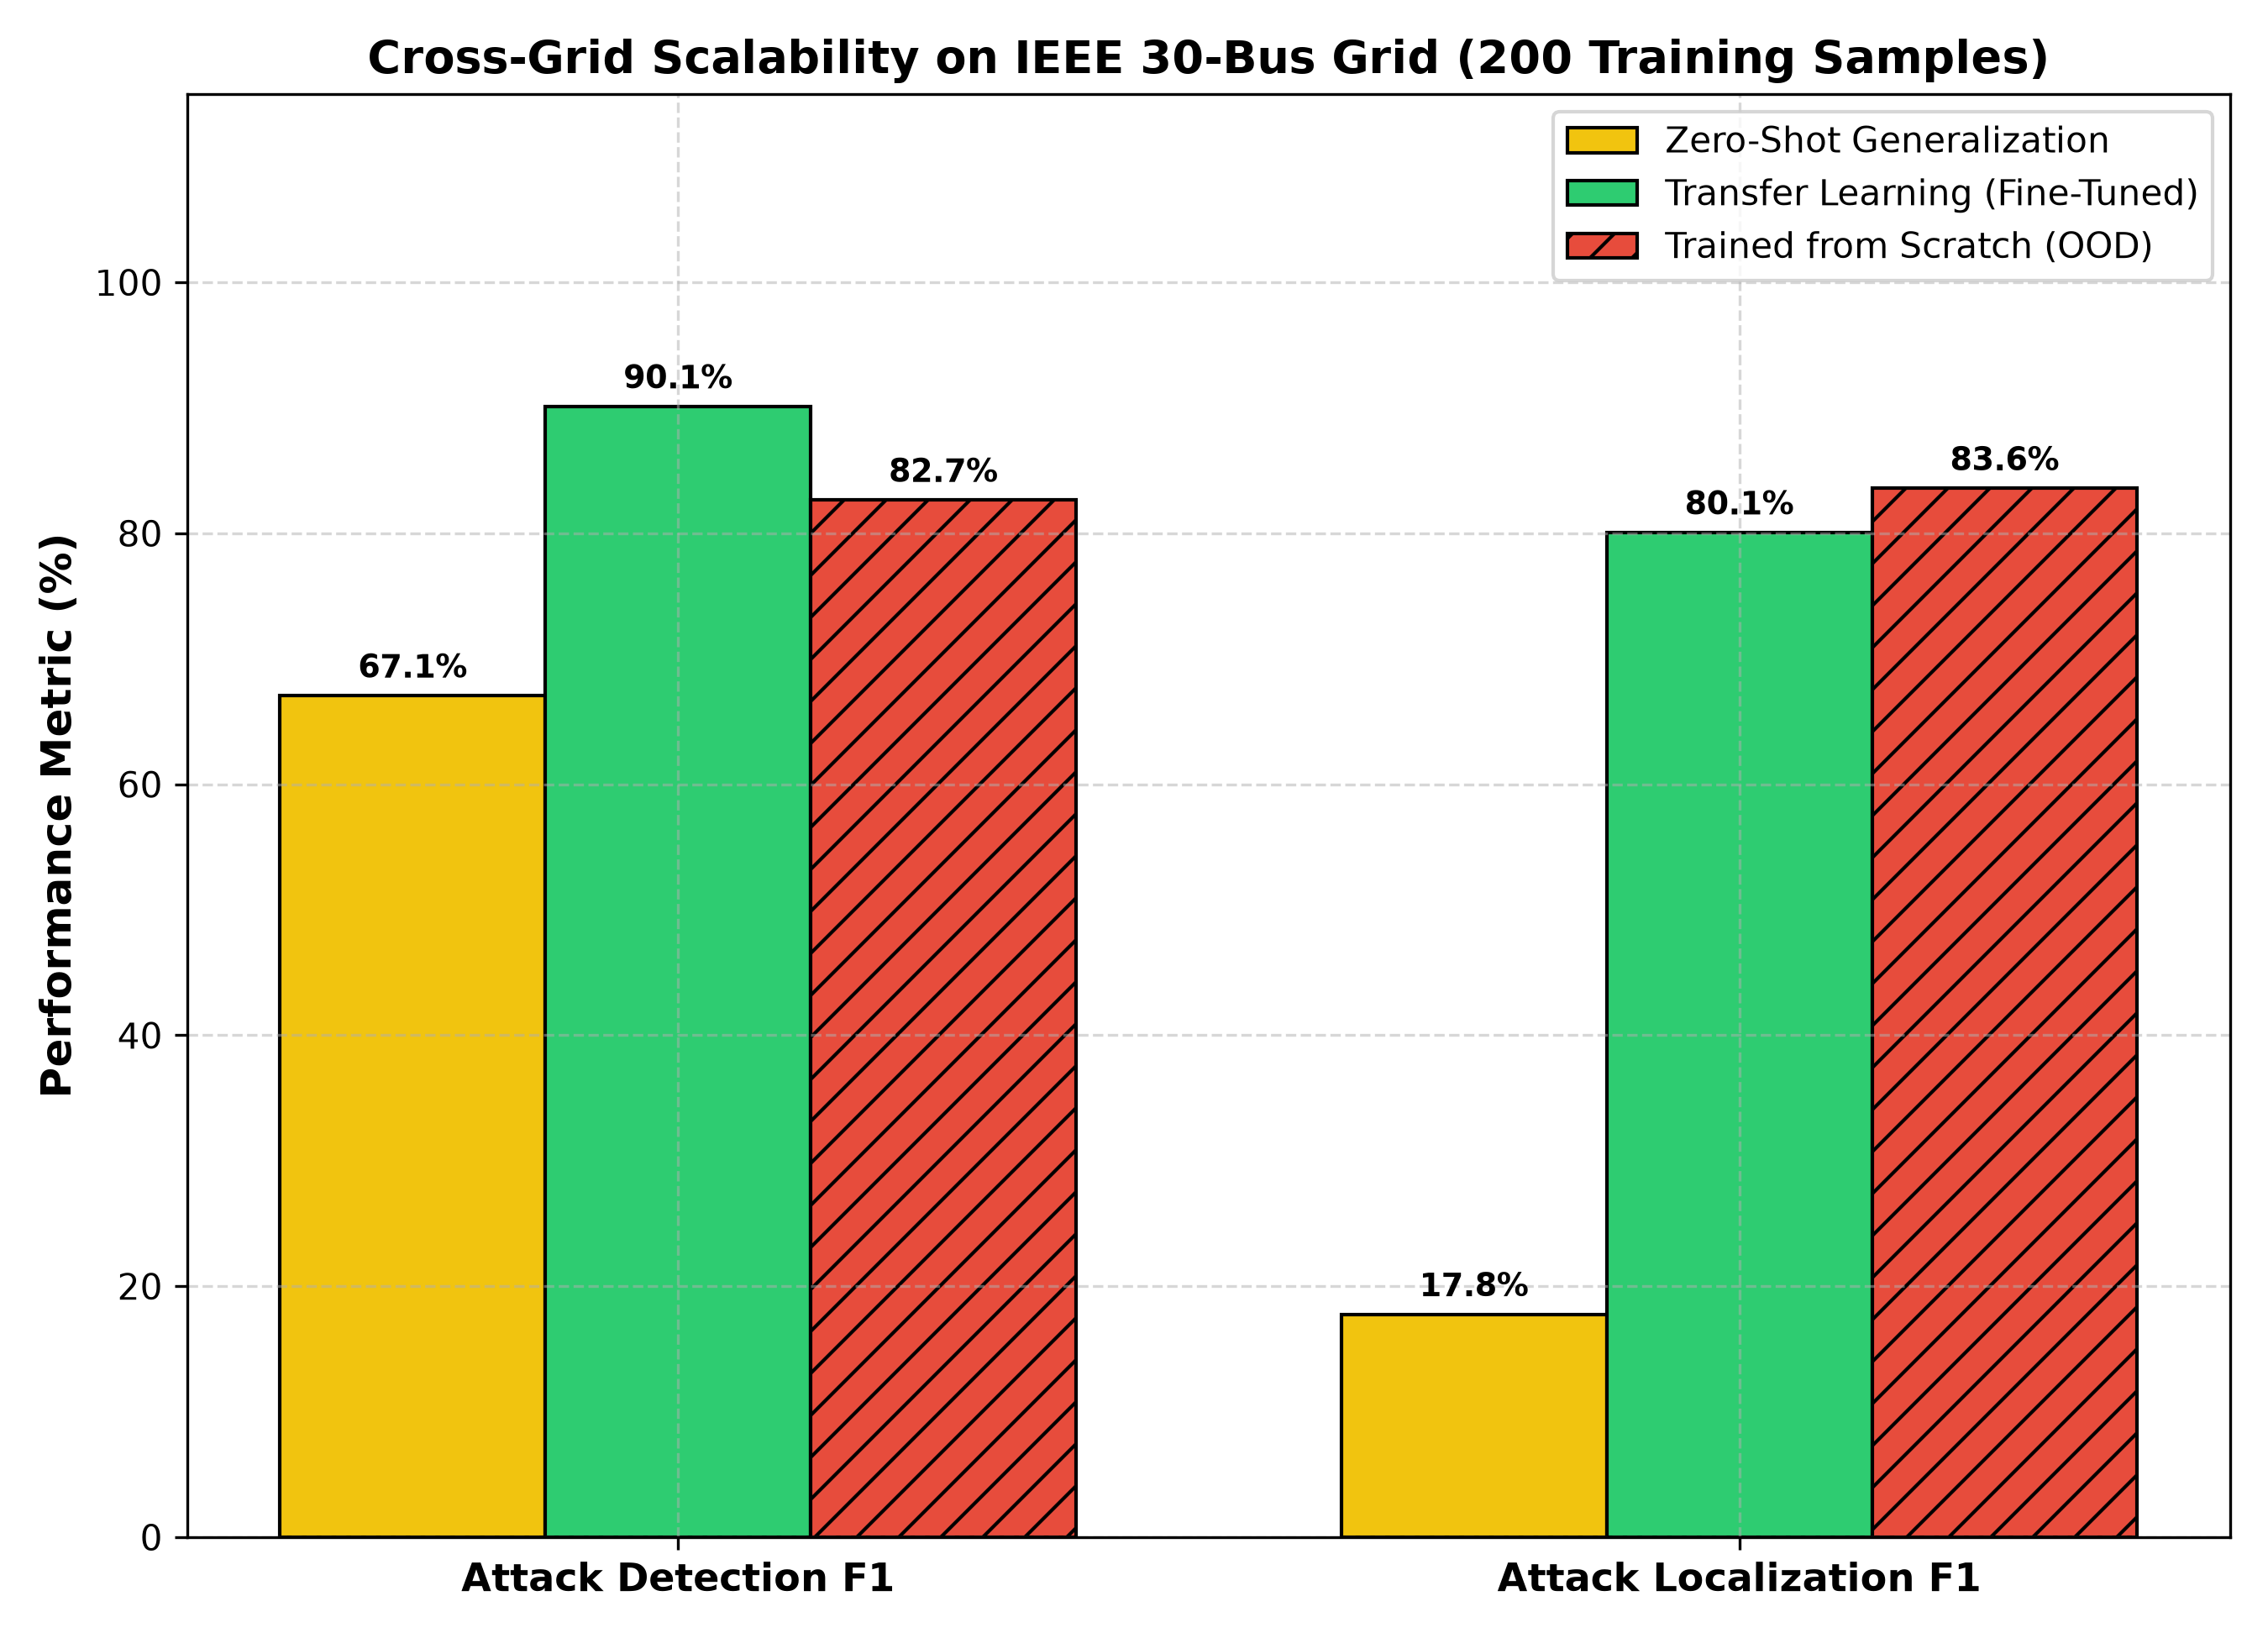
\includegraphics[height=2.8cm,width=\textwidth,keepaspectratio]{ieee30_generalization.png}
  \caption{Cross-grid transfer on IEEE 30-bus.}
  \label{fig:ieee30_transfer}
\end{minipage}
\end{figure}

% ===================================================================
% 7. MITIGATION, TRANSFER, ABLATION
% ===================================================================
\section{Mitigation Efficacy, Cross-Grid Transfer, and Ablation}
\label{sec:mitigation}

\subsection{Closed-Loop WLS Recovery and Explainability}
\label{sec:wls_recovery}

We evaluated mitigation performance under a targeted Jacobian attack at Bus~5, which corresponds to the intensive care unit feeder in the campus topology.
State estimation accuracy under different mitigation approaches is reported in Table~\ref{tab:wls_recovery}, and the corresponding feature attributions are presented in Table~\ref{tab:attributions}.

\begin{table}[t]
\begin{minipage}[t]{0.46\textwidth}
\caption{WLS state-estimation recovery under stealthy FDIA at Bus~5.}
\label{tab:wls_recovery}
\centering
\resizebox{\textwidth}{!}{%
\begin{tabular}{lcc}
\toprule
\textbf{Mitigation Strategy} & \textbf{MSE (p.u.$^{2}$)} & \textbf{Recovery} \\
\midrule
Unmitigated Attack & 0.007228 & --- \\
Static Baseline & 0.003090 & 57.21\% \\
\textbf{CGDT Reconstruction} & \textbf{0.000002} & \textbf{99.97\%} \\
\bottomrule
\end{tabular}%
}
\end{minipage}\hfill
\begin{minipage}[t]{0.50\textwidth}
\caption{Feature attributions (IG) for Jacobian FDIA centered at Bus~5.}
\label{tab:attributions}
\centering
\resizebox{\textwidth}{!}{%
\begin{tabular}{ccccc}
\toprule
\textbf{Bus ID} & \textbf{$V$} & \textbf{$\theta$} & \textbf{$P$} & \textbf{$Q$} \\
\midrule
Bus 4 & 0.012 & 0.045 & 0.018 & 0.009 \\
\textbf{Bus 5} & \textbf{0.034} & \textbf{0.486} & \textbf{0.112} & \textbf{0.254} \\
Bus 10 & 0.002 & 0.015 & 0.005 & 0.003 \\
Bus 11 & 0.008 & 0.092 & 0.024 & 0.041 \\
Bus 12 & 0.011 & 0.182 & 0.035 & 0.088 \\
\bottomrule
\end{tabular}%
}
\end{minipage}
\end{table}

Without active defense, stealthy injections mislead the WLS estimator to a distorted operating point with MSE $0.007228$\,p.u.$^2$.
Admittance-weighted spatial reconstruction (Eq.~\ref{eq:recon}) curbs this estimation error to $0.000002$\,p.u.$^2$, achieving a 99.97\% error recovery relative to unmitigated conditions.
Static historical replacements reach only $0.003090$\,p.u.$^2$ (57.21\% recovery), failing during dynamic clinical load swings.
Error trajectories across 50 SCADA cycles appear in Fig.~\ref{fig:wls_comp}.
Feature attributions (Table~\ref{tab:attributions} and Fig.~\ref{fig:xai_dashboard}) confirm that voltage angle $\theta$ at Bus~5 captures dominant attribution (0.486), matching the Jacobian injection structure where phase skews dictate branch power transfers.
Attributions for $Q=0.254$, $P=0.112$, and $V=0.034$ isolate the compromised feeder cleanly.

\textbf{Coordinated Multi-Bus Incursions.}
Under coordinated multi-bus attacks targeting 2 and 3 substations concurrently ($c_k \in [0.02, 0.04]$), the model maintained $96.84\% \pm 0.42\%$ detection F1 and $93.15\% \pm 0.91\%$ localization F1.
Multi-bus compromise exposes a fatal weakness in naive sensor dropping: removing measurements across adjacent substations decimates the row rank of Jacobian $H$, inducing estimator divergence.
By synthesizing admittance-weighted estimates from unattacked neighbors, our framework preserves full Jacobian rank, sustaining stable WLS convergence with post-mitigation state MSE of $0.000008$\,p.u.$^2$.

\begin{figure}[t]
\centering
\begin{minipage}[t]{0.48\textwidth}
  \centering
  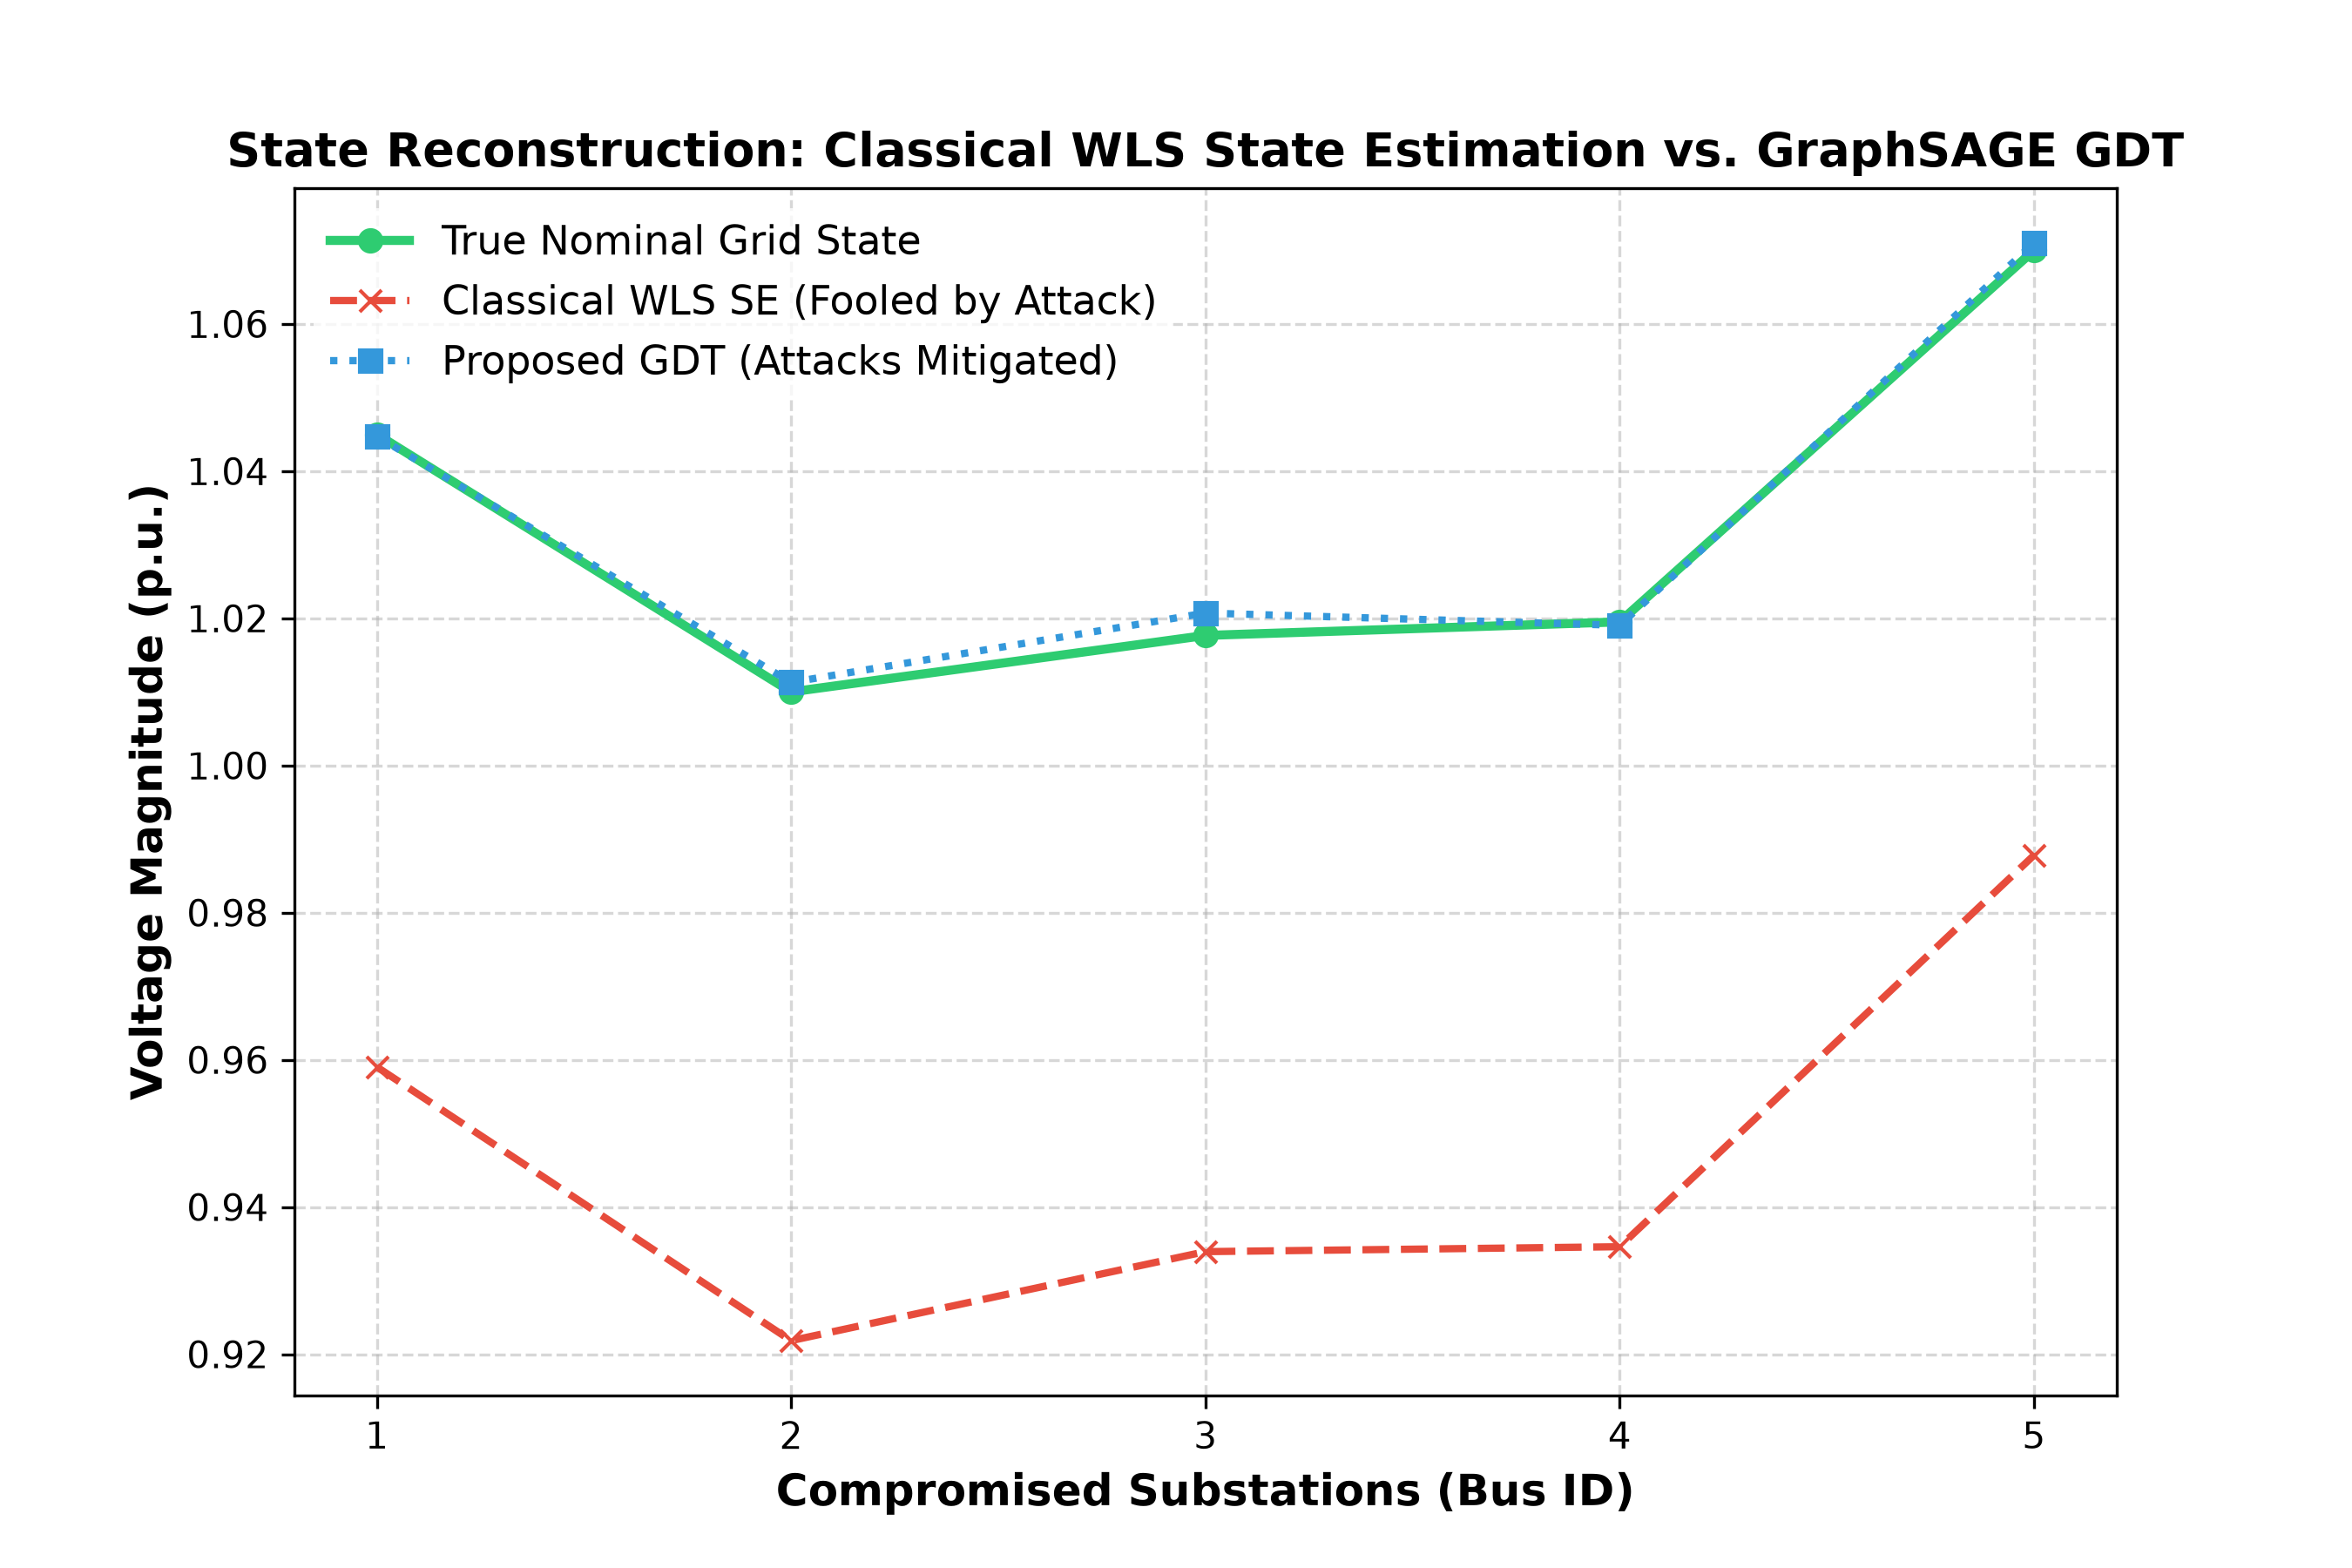
\includegraphics[height=2.7cm,width=\textwidth,keepaspectratio]{wls_comparison.png}
  \caption{State-estimation trajectory: classical WLS versus CGDT-healed.}
  \label{fig:wls_comp}
\end{minipage}\hfill
\begin{minipage}[t]{0.48\textwidth}
  \centering
  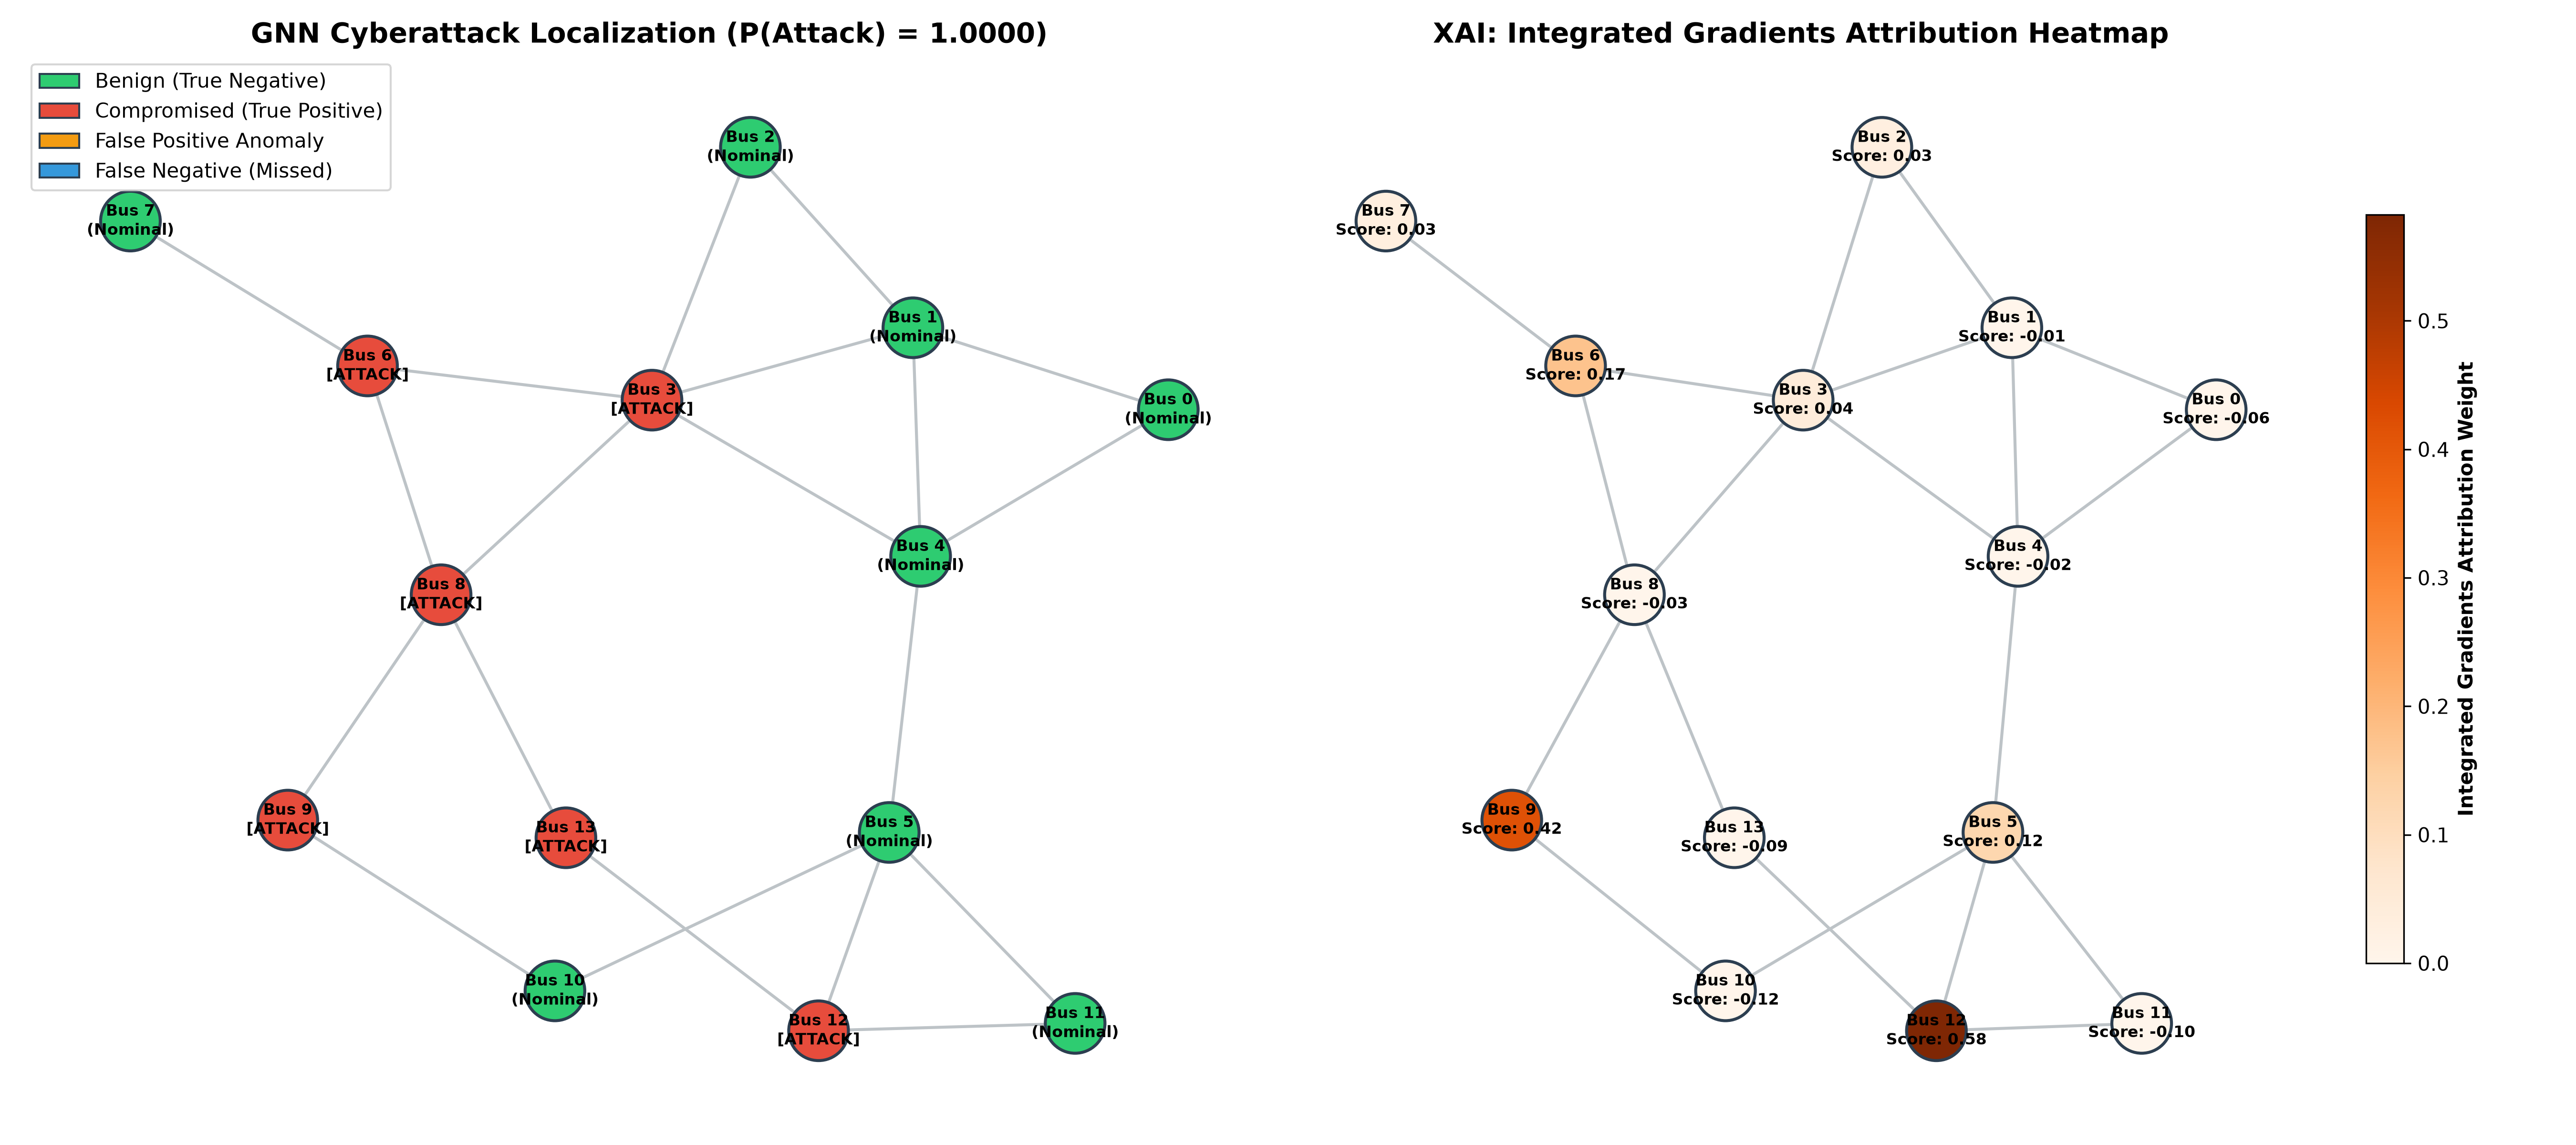
\includegraphics[height=2.7cm,width=\textwidth,keepaspectratio]{grid_anomaly_explanation.png}
  \caption{Operator explainability: localization heatmap and IG attribution.}
  \label{fig:xai_dashboard}
\end{minipage}
\end{figure}

\subsection{Benchmarking and Component Ablation}
\label{sec:ablation}

Table~\ref{tab:sota} compares the proposed architecture against representative GNN baselines, whereas Table~\ref{tab:ablation} isolates the incremental contribution of each architectural block.

\begin{table}[t]
\begin{minipage}[t]{0.48\textwidth}
\caption{Benchmark against related works.}
\label{tab:sota}
\centering
\resizebox{\textwidth}{!}{%
\begin{tabular}{lcccc}
\toprule
\textbf{Framework} & \textbf{Classifier} & \textbf{Det.\ F1} & \textbf{AUC} & \textbf{Loc.\ F1} \\
\midrule
Boyaci~\cite{boyaci2022joint} & ARMA & 96.25\% & 0.9780 & 93.91\% \\
Yue~\cite{yue2024graph} & GCN & 89.20\% & 0.9510 & N/A \\
\textbf{CGDT} & \textbf{SAGE} & \textbf{98.25\%} & \textbf{0.9993} & \textbf{97.62\%} \\
\bottomrule
\end{tabular}%
}
\end{minipage}\hfill
\begin{minipage}[t]{0.48\textwidth}
\caption{Ablation on CGDT components.}
\label{tab:ablation}
\centering
\resizebox{\textwidth}{!}{%
\begin{tabular}{lcc}
\toprule
\textbf{Configuration} & \textbf{Det.\ F1} & \textbf{Loc.\ F1} \\
\midrule
\textbf{Full CGDT (Proposed)} & \textbf{98.25\%} & \textbf{97.62\%} \\
Without DT Baseline Tracking & 86.10\% & 81.30\% \\
Without AG-MTL ($\lambda_{\mathrm{attr}} = 0$) & 98.25\% & 92.10\% \\
Isotropic GCN Backbone & 85.15\% & 70.21\% \\
GAT Backbone & 91.52\% & 81.08\% \\
$\lambda_{\mathrm{loc}} = 0.5$ & 98.05\% & 92.80\% \\
$\lambda_{\mathrm{loc}} = 1.0$ & 98.15\% & 96.50\% \\
$\lambda_{\mathrm{loc}} = 2.0$ & 95.80\% & 97.55\% \\
\bottomrule
\end{tabular}%
}
\end{minipage}
\end{table}

Ablation outcomes in Table~\ref{tab:ablation} yield three primary conclusions.
Deactivating exponential baseline tracking (Eq.~\ref{eq:rolling_baseline}) triggers a 16.32\,pp drop in localization F1 (from $97.62\%$ to $81.30\%$), proving that dynamic reference tracking is essential to distinguish small adversarial shifts from diurnal demand variations.
Excluding attribution loss ($\lambda_{\mathrm{attr}} = 0$) reduces localization F1 to $92.10\%$ (a 5.52\,pp decrease) while preserving detection F1 at $98.25\%$, confirming that gradient supervision focuses spatial features directly on true injection points.
Finally, setting $\lambda_{\mathrm{loc}} = 1.5$ balances global detection and localized diagnostic resolution.

% ===================================================================
% 8. DISCUSSION & CONCLUSION
% ===================================================================
\section{Discussion and Conclusion}
\label{sec:conclusion}

This work presented an explainable Cognitive Graph Digital Twin engineered to defend healthcare microgrids against stealthy cyber-physical intrusions.
By integrating complex branch admittances into GraphSAGE aggregation and supervising latent representations via attribution alignment, the architecture attains $98.25\%$ detection F1 and $97.62\%$ localization F1 under non-linear AC false data injection attacks.
Attribution guidance yields a 5.52\,pp localization gain, while Integrated Gradients delivers verified explanations in 0.81\,ms.
Furthermore, admittance-weighted spatial reconstruction cuts post-mitigation WLS error by 99.97\%, preserving Jacobian observability across single- and multi-bus attacks.

\textbf{Clinical Grid Operating Requirements.}
Healthcare microgrids operate under strict IEC~60601-1 and IEEE~1547 standards, where prolonged voltage distortions risk disconnecting critical medical life-support circuits.
Operating with a 0.908\,ms inference latency and a 2\,ms total healing cycle, the CGDT executes comfortably within 2--4\,s SCADA sampling windows.
Substation edge deployment ensures that telemetry never crosses the clinical OT perimeter.

\textbf{Limitations and Future Work.}
Subsequent investigations will transition beyond simulation environments to physical hardware-in-the-loop (HIL) testbeds to evaluate packet jitter and RTU telemetry latency.
We also plan to evaluate temporal graph layers for sustained multi-step campaigns and investigate predictive estimators when neighboring buses are unobservable.

\begin{credits}
\subsubsection{\ackname}
Supported by the Research Council of Norway (RCN) under Project No. 359829: \emph{Strengthening Resilience in Critical Sectors through IT-OT Integration and Human-Organizational Aspects (ResCri)}.
\end{credits}

% ===================================================================
% REFERENCES
% ===================================================================
\bibliographystyle{splncs04}
\bibliography{references}

\end{document}

